\twocolumn

\part{Introduction}

\section{\hs{}}

Reactive oxygen species (`ROS') such as superoxide (\ce{O2-}) or hydrogen
peroxide (\ce{H2O2}) are toxic to the body, causing damage to proteins or DNA,
with links to various diseases including cancer. As such organisms under
aerobic conditions counteract ROS via eg Superoxide Dismutase (`SOD') which
catalyses the partitioning of superoxide into molecular oxygen and hydrogen
peroxide.

One major source of superoxide is the oxidative phosphorylation within the
mitochondrial matrix. \cite{Novo2008} To a lesser extent these superoxides
diffuse into the cytoplasm, where they are acted upon by SOD. A significant
portion of superoxides however is oxidised by superoxide oxidases - hence after
referred to as `SOO' or `Halonsaft' due to its colour - a family of
membrane-bound proteins which oxidise superoxides.\cite{superoxide_salvaging}.

One protein of this family is CybB from \ecoli{} which was shown to function as
a membrane-embedded superoxide:ubiquinone oxidoreductase. It oxidises
superoxide to oxygen while simultaneously reducing quinone to
quinol.\cite{superoxide_salvaging} This enzymatic activity both serves to
remove superoxides in close proximity to the cell membrane, as well as restore
the quinone pool, helping to save energy.

\hs{} contains two Hemes which are known to play an important role in its
ability to transfer electrons from one side of the membrane to the other,
thereby oxidising superoxides to molecular oxygen and reducing quinone to
quinol.\cite{superoxide_salvaging} Such interactions are visualized in figure
\ref{fig:superoxide_activity}.

\hs{} further contains a highly-conserved Histidine at position 158 which is
conjectured to play a role as an electron donor for its enzymatic activity.
Mutations of this amino acid might have an effect on the ability of the enzyme
to interact with its substrates.\cite{superoxide_salvaging}

Regulation of \hs{} in \ecoli{} was shown to not depend on the presence or
absence of oxygen, and to lead to significantly higher expression during the
stationary phase of bacterial growth.\cite{superoxide_salvaging}

\begin{figure}
	\centering
	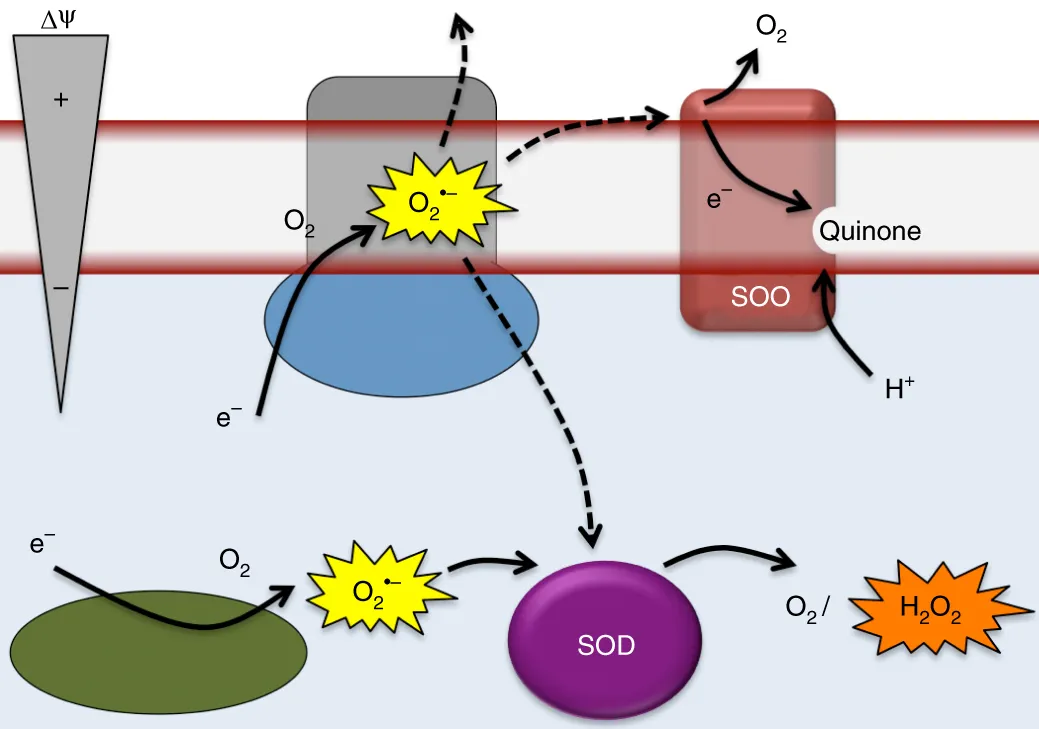
\includegraphics[width=\linewidth]{../img/superoxide_activity.png}
	\caption{Proposed interaction between superoxide oxidase, superoxide dismutase and superoxide-producing membrane-bound systems from \cite{superoxide_salvaging}}
	\label{fig:superoxide_activity}
\end{figure}

\section{Protein expression in \ecoli{}}

Protein expression in \ecoli{} is used for many purposes, such as obtaining
large amounts of proteins for crystal structure analysis or for analysing
activity of enzymes. In the case of membrane-bound proteins, detergent is
required to remove proteins from cell membranes. In the case of proteins which
are expressed only in small concentrations, the required cell volume and
thereby required detergent can become large, increasing cost of protein
purification.\cite{memstar}

While LB is one of the most popular media for protein expression with \ecoli{},
other media and techniques exist to achieve either a larger number of cells or
higher concentration of membrane proteins per cell.
